\subsection{Rank-Two Design Transfer in Eight Dimensions}
To test compression beyond rank one, we fix $d=8$ and $K=2$. Define
\begin{equation}
\Sigma=\operatorname{diag}(8,5,3,2,1,1,1,1).
\end{equation}
Generate $600$ independent vectors $X_j\sim\mathcal N(0,\Sigma)$ and set $u_j=X_j/\|X_j\|$, with $u_{ji}$ denoting coordinate $i$ of direction $u_j$. The finite law assigns weights proportional to $\exp(0.6u_{j1}+0.4u_{j2}u_{j3})$. This realized finite law, not the underlying continuous Gaussian construction, is the target of compression. Reproduction uses seed $20260920$ with separate streams for directions, linear-program objectives, candidate projectors, and moment checks.

For matching orders $r=1,2$, positive linear programs preserve every homogeneous monomial of degree $2r$, together with total mass. Denote the resulting order-$r$ compressed law by $\nu_r$. Refined solutions retain $36$ and $330$ directions, respectively. At $r=3$, the support bound $D_{8,3}=1716$ exceeds the original $600$ directions, so we retain the original law as a reference rather than claim further compression. Checks on $128$ fresh projectors for each of ranks $2$ and $4$ give maximum coverage-moment residual $\RankResidual$. Thus the same surrogate weights are tested at more than one rank.

For each $\gamma\in\{1,10\}$, define a common finite candidate family $\mathcal Q_\gamma\subset\Pset$. It contains $512$ Haar projectors, the leading covariance projector, and $12$ projectors refined by projected-gradient ascent with orthonormalization. The refinements use four common starts for each of the original law and the two compressed laws. The resulting $\RankCandidates$ candidates are shared by all matching orders. Let $\widehat P_r$ maximize surrogate information over $\mathcal Q_\gamma$. Define the candidate-family information error $E_r^{\mathcal Q}$ and transfer regret $R_r^{\mathcal Q}$ by
\begin{align}
E_r^{\mathcal Q}&=\max_{P\in\mathcal Q_\gamma}|\I_\mu(P;\gamma)-\I_{\nu_r}(P;\gamma)|,\\
R_r^{\mathcal Q}&=\max_{P\in\mathcal Q_\gamma}\I_\mu(P;\gamma)-\I_\mu(\widehat P_r;\gamma).
\end{align}
These are the maximum error and transfer regret within the finite family. Exhaustive evaluation verifies $R_r^{\mathcal Q}\le2E_r^{\mathcal Q}$. The same comparison underlying Theorem~\ref{thm:representation}(a)--(b) applies to this restricted family, but these numerical values are not continuous-projector suprema or certified global-optimum regrets.

At $r=2$ and $\gamma=10$, the candidate information error is $\RankError$ nats and transfer regret is $\RankRegret$ nats. Figure~\ref{fig:rank_transfer} reports both quantities versus matching order. The third-order reference reproduces the original objective up to rounding because it uses the original law. This example directly tests measurement transfer for $K>1$ and also illustrates why an existence bound need not provide useful compression at every dimension and order.
\begin{figure}[t]
\centering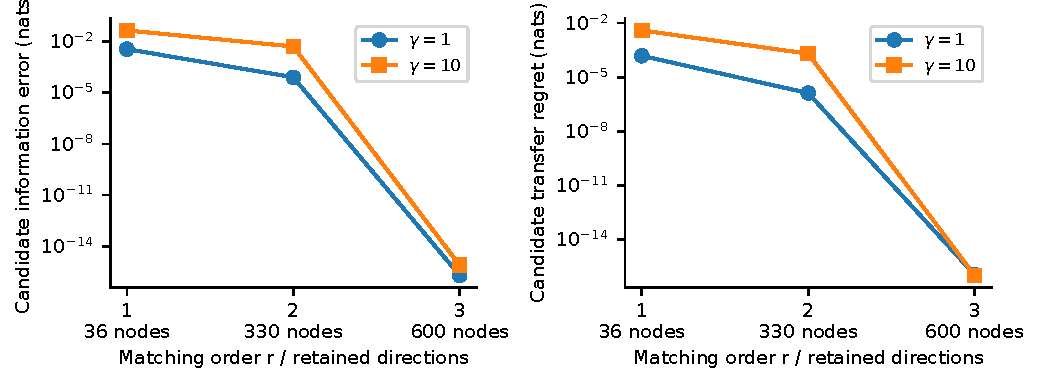
\includegraphics[width=0.95\textwidth]{figures/fig_rank_transfer.pdf}
\caption{Eight-dimensional rank-two design transfer over a common finite candidate family. Orders one and two use compressed laws; order three retains the original 600-direction law. Values below $10^{-16}$ are displayed at that floor. The curves do not certify optimization over all rank-two projectors.}
\label{fig:rank_transfer}
\end{figure}
